\documentclass{standalone}
\usepackage{tikz}
\usepackage{amsmath}

\begin{document}

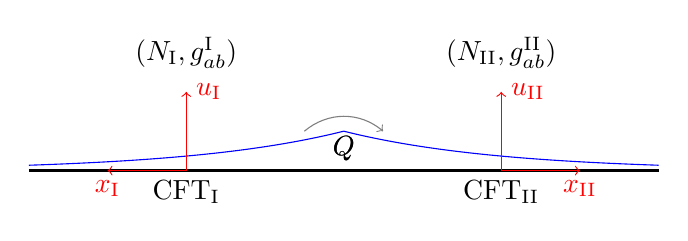
\begin{tikzpicture}

    % Draw the CFT lines
    \draw[thick] (-4,0) -- (0,0) node[pos=0.5, below] {CFT$_{\text{I}}$};
    \draw[thick] (0,0) -- (4,0) node[pos=0.5, below] {CFT$_{\text{II}}$};

    % Draw the curved interface brane Q
    \draw[domain=-4:0, smooth, variable=\x, blue] 
        plot ({\x}, {0.5*exp(\x/2)}) node[pos=0.7, above, black] {$Q$};
    \draw[domain=0:4, smooth, variable=\x, blue] 
        plot ({\x}, {0.5*exp(-\x/2)}) node[pos=0.3, above, black] {$Q$};

    % Draw the red vectors
    \draw[red, ->] (-2,0) -- (-2,1) node[right] {$u_{\text{I}}$};
    \draw[red, ->] (-2,0) -- (-3,0) node[below] {$x_{\text{I}}$};

    \draw[red, ->] (2,0) -- (2,1) node[right] {$u_{\text{II}}$};
    \draw[red, ->] (2,0) -- (3,0) node[below] {$x_{\text{II}}$};

    % Labels for the bulks
    \node at (-2,1.5) {$(N_{\text{I}}, g^{\text{I}}_{ab})$};
    \node at (2,1.5) {$(N_{\text{II}}, g^{\text{II}}_{ab})$};

    % Curved arrow between Qs
    \draw[gray, ->] (-0.5,0.5) to [bend left=40] (0.5,0.5);

\end{tikzpicture}

\end{document}